\begin{center}
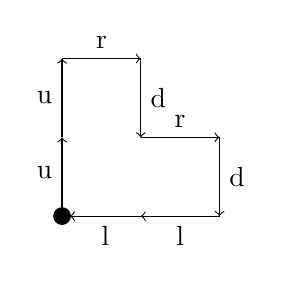
\begin{tikzpicture}
    \filldraw[black] (0,0) circle (3pt);
    \draw[->] (0,0.1) -- (0,1) node[midway,left] {\str{u}}; 
    \draw[->] (0,1) -- (0,2) node[midway,left] {\str{u}};
    \draw[->] (0,2) -- (1,2) node[midway,above] {\str{r}};
    \draw[->] (1,2) -- (1,1) node[midway,right] {\str{d}}; 
    \draw[->] (1,1) -- (2,1) node[midway,above] {\str{r}};
    \draw[->] (2,1) -- (2,0) node[midway,right] {\str{d}}; 
    \draw[->] (2,0) -- (1,0) node[midway,below] {\str{l}}; 
    \draw[->] (1,0) -- (0.1,0) node[midway,below] {\str{l}}; 
\end{tikzpicture}
\end{center}